\documentclass[tikz]{standalone}
\begin{document}
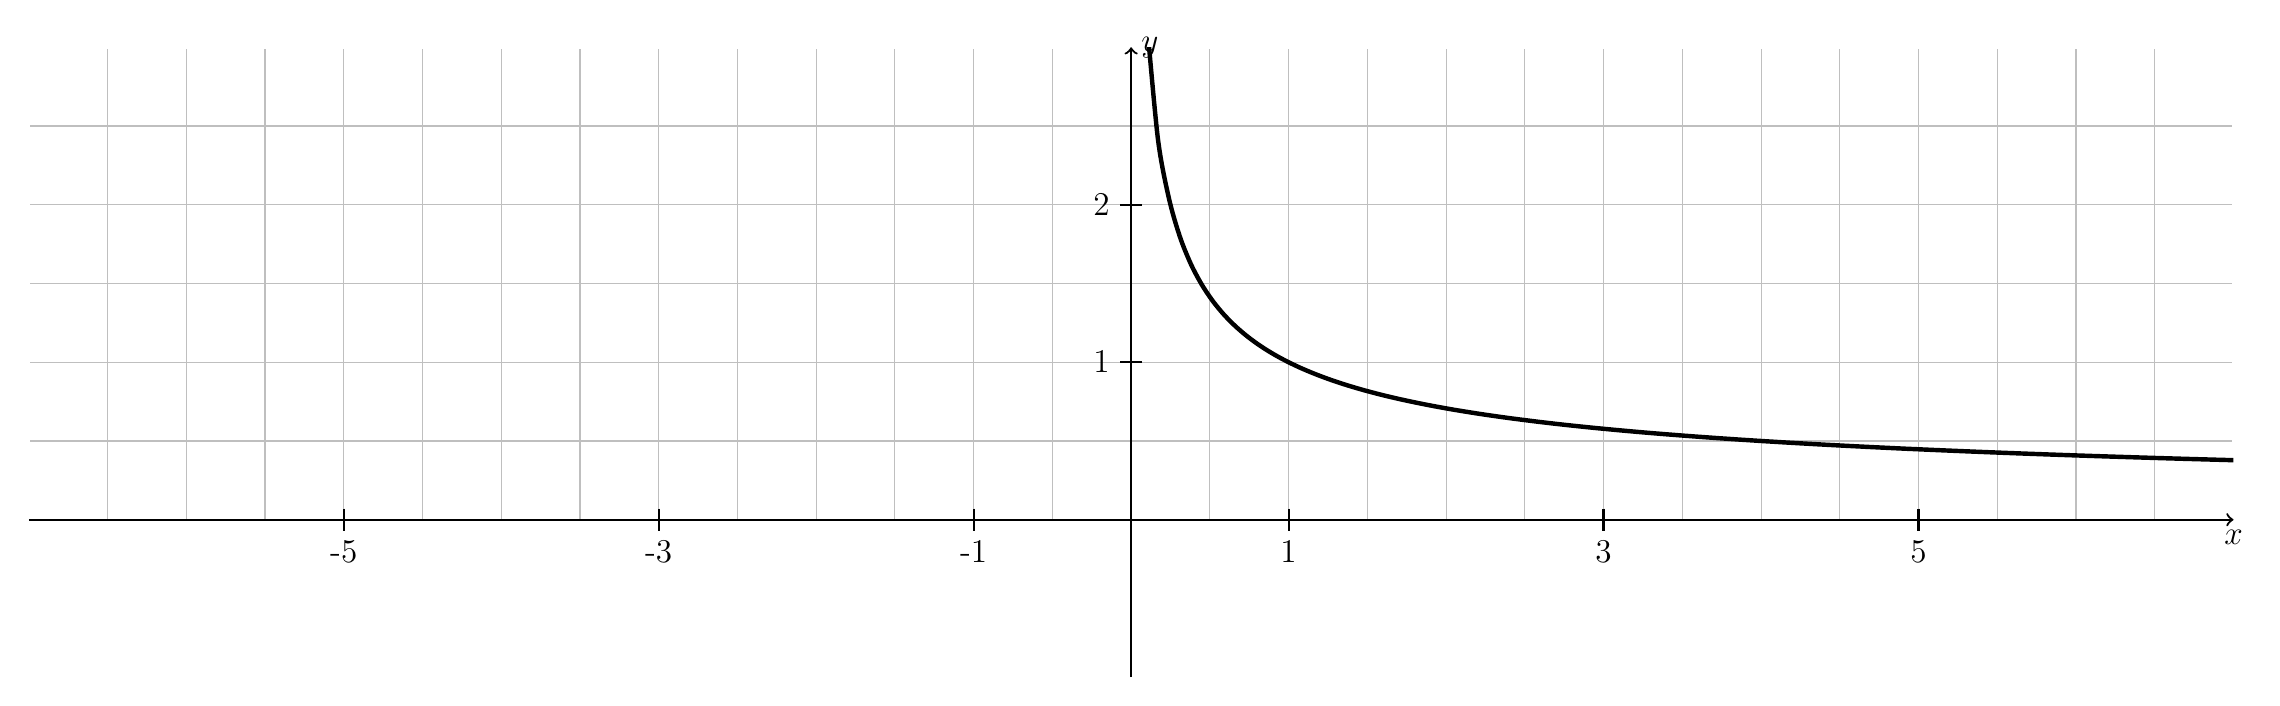
\begin{tikzpicture}[scale=2]
\tikzstyle{every node}=[font=\large]
 
% create a white background, with a black frame
%\draw [fill=white] (-7.5,-1.5) rectangle (7.5,3.5); 

% draw a grid
\draw[step=5mm, lightgray, thin] (-6.99,0) grid (6.99,2.99); 
%\draw[step=1cm, gray] (0,-0) grid (6.5,3.5); 

% draw axes
\draw [->,thick] (-7,0) -- (7,0) node[below] {$x$}; 
\draw [->,thick] (0,-1) -- (0,3) node[right] {$y$};

% tick marks
\foreach \x in {-5,-3,-1,1,3,5} 
	\draw [thick] (\x cm,2pt) -- (\x cm,-2pt) node[below] {\x};
\foreach \y in {1,2} 
	\draw [thick] (2pt,\y cm) -- (-2pt,\y cm) node[left] {\y};

% plot curve
\clip (-7,-1) rectangle (7,3);
\draw[ultra thick,domain=0.1:7,smooth,samples=100] plot (\x,{1/pow(\x,0.5)});

\end{tikzpicture}
\end{document} 
